\documentclass[10pt,twocolumn,letterpaper]{article}

\usepackage{cvpr}
\usepackage{times}
\usepackage{epsfig}
\usepackage{graphicx}
\usepackage{amsmath}
\usepackage{amssymb}
\usepackage{tabularx} 
% Include other packages here, before hyperref.

% If you comment hyperref and then uncomment it, you should delete
% egpaper.aux before re-running latex.  (Or just hit 'q' on the first latex
% run, let it finish, and you should be clear).
\usepackage[pagebackref=true,breaklinks=true,letterpaper=true,colorlinks,bookmarks=false]{hyperref}

\cvprfinalcopy % *** Uncomment this line for the final submission

\def\cvprPaperID{****} % *** Enter the CVPR Paper ID here
\def\httilde{\mbox{\tt\raisebox{-.5ex}{\symbol{126}}}}

% Pages are numbered in submission mode, and unnumbered in camera-ready
\ifcvprfinal\pagestyle{empty}\fi
\begin{document}

%%%%%%%%% TITLE
\title{Task 5, Task 6, Task 7: Segmentation \& Localization }

\author{Konstantinos Katergaris\\
Arizona State University\\
1151 S Forest Ave, Tempe, AZ\\
{\tt\small kkaterga@asu.edu}}

%\thispagestyle{empty}

\maketitle

\section{Task 5}

\subsection{Introduction}
In this section, the task was to perform semantic segmentation on lungs given a chest X-ray. To achieve this, a DeepLabV3 model with a ResNet101 backbone was used. This yielded an average Dice Score of 0.9734, an average IoU of 0.9481, an average Precision of 0.9731, and an average Recall of 0.9737. However, to achieve better results, two augmentation experiments were conducted: one with light augmentations and the other with heavy augmentations. It was hypothesized that the light augmentation would perform better, as the heavy augmentations might be too intense.
\subsection{Dataset}
The dataset\cite{DatasetForClass} consists of 60 chest x-rays and their subsequent lung masks given by a binary image. A custom dataset was made to load these images.

\subsection{Training}
The model's backbone was frozen. Furthermore, a learning rate of 0.001 and a ReduceLROnPlateau scheduler with a factor of 0.1 and a patience of 5 were used. Additionally, the model was trained for 50 epochs with a batch size of 16. A combination of dice loss and binary cross-entropy (BCE) was calculated and scaled down so that each contributed equally to the final loss, with a 50\% weighting.

\subsection{Experiments}
To test if data augmentations would help the results of the model albumentations transforms library was used. The following augmentation where applied to the both the light and heavy augmentations: Horizontal Flip, Random Rotate 90, Normalization with mean=[0.485, 0.456, 0.406] and std=[0.229, 0.224, 0.225]. The heavy augmentations added the following augmentations: GridDistortion, ShiftScaleRotate, RandomBrightnessContrast, CLAHE, GaussianBlur, and GaussNoise.



\subsection{Results}
The following Tables ~\ref{tab:dice_score_results}  ~\ref{tab:iou_results} ~\ref{tab:precision_recall_results} compare the performance of the model under three training scenarios: without augmentations, with light augmentations, and with heavy augmentations. The metrics reported are the average Dice Score, average IoU, average Precision, and average Recall. 
\begin{table}[h!]
\centering
\begin{tabular}{l|c|}
\hline
\bf{Training Condition} & \bf{Dice Score} \\ \hline
No Augmentation & 0.9734 \\ \hline
Light Augmentation & 0.9743 \\ \hline
Heavy Augmentation & 0.9717 \\ \hline
\end{tabular}
\caption{Comparison of Dice Score Across Different Augmentation Strategies}
\label{tab:dice_score_results}
\end{table}

\begin{table}[h!]
\centering
\begin{tabular}{l|c|}
\hline
\bf{Training Condition} & \bf{IoU} \\ \hline
No Augmentation & 0.9481 \\ \hline
Light Augmentation & 0.9499 \\ \hline
Heavy Augmentation & 0.9449 \\ \hline
\end{tabular}
\caption{Comparison of IoU Across Different Augmentation Strategies}
\label{tab:iou_results}
\end{table}

\begin{table}[h!]
\centering
\begin{tabular}{l|c|c|}
\hline
\bf{Training Condition} & \bf{Precision} & \bf{Recall} \\ \hline
No Augmentation & 0.9731 & 0.9737 \\ \hline
Light Augmentation & 0.9729 & 0.9757 \\ \hline
Heavy Augmentation & 0.9691 & 0.9742 \\ \hline
\end{tabular}
\caption{Comparison of Precision and Recall Across Different Augmentation Strategies}
\label{tab:precision_recall_results}
\end{table}


\subsection{Conclusion}
Aligned with the hypothesis, the light augmentations performed the best. Furthermore, it is hypothesized that the heavy augmentations performed the worst because they were too difficult for the model to learn given the limited data.
\newpage

\section{Task 6}

\subsection{Introduction}
In this section, the task was to perform instance segmentation on lungs given a chest X-ray. A Mask R-CNN model with a ResNet50-FPN backbone was used. The model achieved an average IoU of 0.9354, an average Precision of 0.9571, and an average Recall of 0.9763 after 20 epochs.

\subsection{Dataset}
The dataset used for this task \cite{DatasetForClass} consists of 247 chest X-ray images in BMP format, with each X-ray having an associated mask encoded with specific pixel values to represent different anatomical regions: lung field area (255), heart (85), outside lung field (170), and outside body (0). To prepare the data for instance segmentation, a custom data loader was implemented in PyTorch, which handles both the X-ray images and their masks. The images are converted to RGB format, normalized, and then augmented using the Albumentations library. For training random 90-degree horizontal and vertical augmentations were used. Each mask was converted into its corresponding class indices based on the pixel values. Once remapped to integer labels, binary masks are generated for each class using OpenCV's cv2.findContours() method and bounding boxes where made using the boundingRect().


\subsection{Training}
The Mask R-CNN model was initialized with pre-trained weights from the COCO dataset, and the architecture was modified to predict five classes: background, heart, outside lung field, right lung, and other regions. A learning rate of 0.0001 was chosen, and the model was optimized using the Adam optimizer. The default loss function was used. The model was trained by 20 epochs. It is important to note that the epoch with the best validation IoU was saved for evaluation. Furthermore, the Adam optimizer was used.

\subsection{Evaluation}
The model was evaluated on the test set after each epoch using three metrics: Intersection over Union (IoU), Precision, and Recall. Predictions were filtered based on a confidence score threshold of 0.5.

\subsection{Results}
The following table ~\ref{tab:model_performance} shows the results of the model:

\begin{table}[h!]
    \centering
    \begin{tabular}{l|c|}
        \hline
        \bf{Metric} & \bf{Value} \\ \hline
        Average IoU & 0.9354 \\ \hline
        Average Precision & 0.9571 \\ \hline
        Average Recall & 0.9763 \\ \hline
    \end{tabular}
    \caption{Performance metrics of the model after 20 epochs.}
    \label{tab:model_performance}
\end{table}


\section{Task 7}

\subsection{Introduction}
In this section, the task was to perform localization on the heart, and lungs given a chest X-ray. To achieve this, instead of using deep learning the findCountours method in cv2 was used. Surprisingly, this was an effective method.
\subsection{Dataset}
The dataset \cite{DatasetForClass} consists of 247 chest X-ray images in BMP format. The subsequent masks were encoded with the following pixel values: lung field area: 255, heart: 85, outside lung field: 170, and outside body: 0.

\subsection{Implementation}
Each pixel value was converted into a binary mask using the cv2.inRange() function. Furthermore, the cv2.findContours() method was used to find the boundaries of each mask. Lastly, a bounding box was created using the cv2 boundingRect() function. To further differentiate the right and left lungs, each bounding box was compared to the middle x-coordinate of the image. If the width of the bounding box was less than the middle x-coordinate, it was partitioned as the left lung; otherwise, it was partitioned as the right lung.
\subsection{Results}
The results can be found in the following Figure ~\ref{fig:male_local} and ~\ref{fig:female_local}
\begin{figure}[h!]
    \centering
    
\includegraphics[width=1\linewidth]{bounding_boxes_case001_label.png}
    \caption{Localization of lungs and heart on male chest x-ray}
    \label{fig:male_local}
    \end{figure}
\begin{figure}[h!]
    \centering
    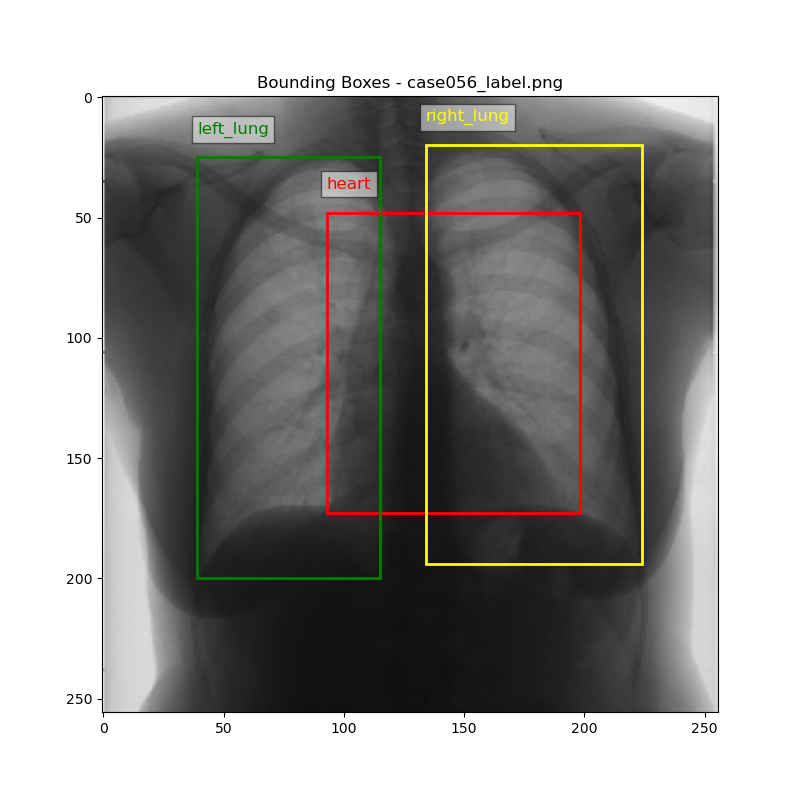
\includegraphics[width=1\linewidth]{bounding_boxes_case056_label.png}
    \caption{Localization of lungs and heart on female chest x-ray}
    \label{fig:female_local}

\end{figure}

{\small
\bibliographystyle{ieee_fullname}
\bibliography{egbib}

}
\end{document}
